\chapter{Software Architecture Design}
\label{chap:software-architecture-design}

\section{System Architecture Overview}
\label{section:architecture-overview}

Sonar Retina utilizes an \textbf{Asynchronous Service-Based Architecture} to meet the real-time processing demands of acoustic accessibility. 
Unlike traditional sequential pipelines, this design decouples the sound capture from the analytical processing, allowing multiple specialized services to run in parallel on separate execution threads.

As illustrated in Figure~\ref{fig:sys-arch}, the architecture consists of three primary layers:
\begin{itemize}
    \item \textbf{Ingestion Layer:} The \textit{Audio Stream Dispatcher} captures raw PCM data from the microphone array and broadcasts it to independent buffers which also has \textit{Audio Processor} to transform data before it reaches service layer.
    \item \textbf{Service Layer:} Two concurrent services—the \textit{SSL Service} (calculating distance via Spectrogram and IPD) and the \textit{SED Service} (identifying sound types via YAMNet)—process the same audio window simultaneously.
    \item \textbf{Presentation Layer:} The \textit{Data Fusion Engine} synchronizes the outputs based on high-resolution timestamps and updates the \textit{Radar UI} for the user.
\end{itemize}

\begin{figure}[ht]
    \centering
    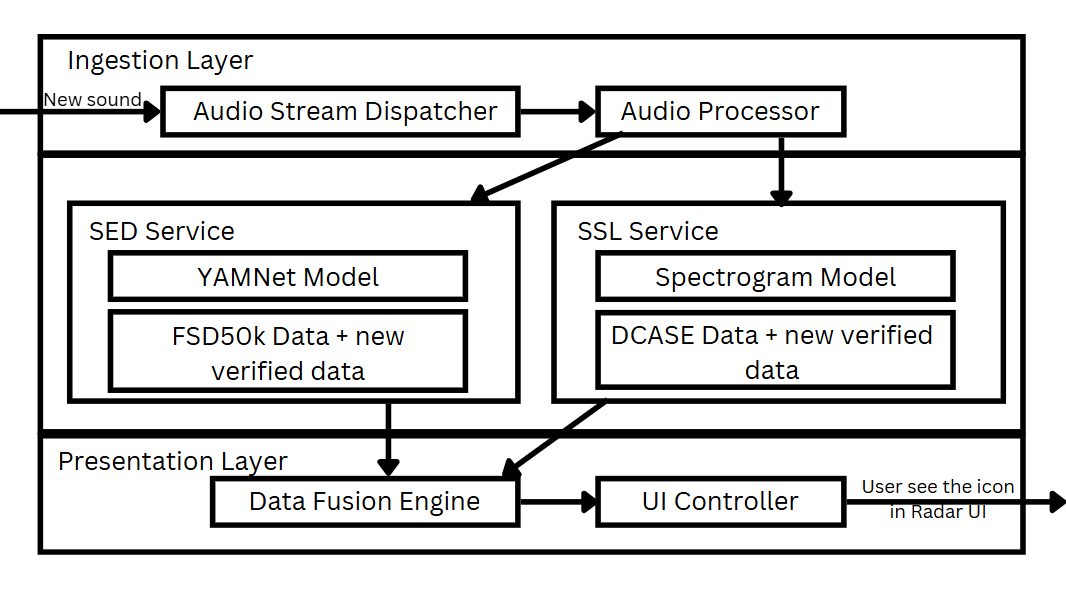
\includegraphics[width=0.9\textwidth]{assets/architecture/system-architecture.png} 
    \caption{Sonar Retina Asynchronous Service-Based Architecture.}
    \label{fig:sys-arch}
\end{figure}

\section{Software Design}
\label{section:software-design}

The runtime behavior of the system follows a \textbf{Reactive Producer-Consumer pattern}. 
The sequence of interactions for a typical sound event—such as a door knock—is detailed below.

\begin{enumerate}
    \item The \textit{Audio Dispatcher} pushes a 1024-sample window to the \textit{Audio Processor}.
    \item The \textit{Audio Processor} prepares the data to match each service format then sends to \textit{Service Layer}.
    \item The \textit{SSL Service} extracts spectrogram and Interaural Phase Difference (IPD) features from the stereo audio stream and classifies the sound proximity into discrete categories (\textit{Near, Medium, Far}) represented as $D$.
    \item Concurrently, the \textit{SED Service} generates a classification label $L$ and a confidence score $C$.
    \item The \textit{Data Fusion Engine} validates that $C > 0.5$ and pairs $D$ with $L$.
    \item The \textit{UI Controller} maps these polar coordinates to a visual icon on the radar view.
\end{enumerate}

\section{AI and Data Design}
\label{section:ai-data-design}

\subsection{Data Sources and Collection}
Our model training and validation rely on the FSD50k and DCASE dataset. 
FSD50k dataset provides over 50,000 excerpts across 200 classes for SED model. 
On the other hand, DCASE dataset is a dataset for SSL model which provides over 1200 audio clips including background noise, reverberation and multiple sound sources.

Data preparation involves converting raw 1D waveforms into Log-Mel Spectrograms (2D time-frequency representations). 
This transformation allows the model to treat audio classification as a pattern recognition task, which is more computationally efficient for deep learning architectures.
Moreover, it allows the model to classify the distance from the processed data.

\subsection{Model Design}
The system utilizes a dual-model approach to concurrently identify and localize acoustic events.

\subsubsection{Sound Event Detection (SED) Model}
We implemented a quantized version of YAMNet, a pre-trained Deep Neural Network based on the MobileNetV1 architecture, for the SED service. 

\textbf{Design Decision:} YAMNet was selected over traditional CNNs due to its use of \textit{depthwise separable convolutions}, which significantly reduces the floating-point operations (FLOPs) required per inference. We utilized TensorFlow Lite (TFLite) 8-bit quantization to ensure the model runs on the device’s mobile hardware without exceeding thermal limits, maintaining a low-latency "Sound-to-Insight" pipeline.

\subsubsection{Sound Source Localization (SSL) Model}

For the SSL service, we implemented a lightweight spectrogram-based localization model utilizing Interaural Phase Difference (IPD) features extracted from stereo microphone input. 
The model estimates the relative proximity of sound sources by analyzing phase differences and frequency-domain spatial characteristics between audio channels.

The preprocessing pipeline converts stereo audio streams into Log-Mel Spectrogram representations while simultaneously extracting IPD features across frequency bins. 
These combined features are then used to classify sound proximity into three discrete categories: \textit{Near}, \textit{Medium}, and \textit{Far}.

\textbf{Design Decision:} 
The spectrogram-IPD approach was selected over traditional Time Difference of Arrival (TDOA) and GCC-PHAT methods due to its improved robustness in noisy and reverberant indoor environments. 
By leveraging frequency-domain spatial representations, the model can better preserve directional cues while remaining computationally lightweight enough for real-time mobile inference.

To maintain low system latency and improve user interpretability, the localization output is simplified into categorical proximity zones rather than continuous spatial coordinates. 
This reduces computational overhead while still providing meaningful environmental awareness for accessibility-focused interaction.
\subsection{Evaluation}
To measure the success of the AI components, we use the following metrics:
\begin{itemize}
    \item \textbf{Mean Average Precision (mAP):} To evaluate the classification accuracy of the SED service across filtered classes. We define the success criteria to be at least 0.75 to balance the false positive result.
    \item \textbf{Categorical Distance Accuracy:} Since the \textbf{SSL Service} maps proximity into three discrete zones (\textit{Far, Medium, and Near}), we evaluate performance using a \textbf{Confusion Matrix}. The goal is to minimize "Critical Errors," defined as the system misidentifying a "Near" sound as "Far" which could pose a safety risk to the user. Therefore, we define that it can occur less than 10%.
    \item \textbf{System Latency:} To maintain "social synchronicity," the total time from microphone input to UI update must be minimal. We set a target threshold of $<500$ms for the 90th percentile (P90) of latency. Measuring the 90\% quantile ensures that the user experience remains smooth and predictable, even during peak computational loads on the mobile hardware.
\end{itemize}